\section{Hardware Used}
\begin{table}[H]
\centering
\caption{All the hardware \& Physical systems used.}
\label{tab:hardware}
\begin{tabular}{|L{3cm}C{3cm}C{6cm}R{3cm}|}
\rowcolor{primary}
\textcolor{white}{\textbf{Hardware}} & \textcolor{white}{\textbf{Picture}} & \textcolor{white}{\textbf{Specifications}} & \textcolor{white}{\textbf{Usage}} \\
\hline
Workstation A (Desktop) & 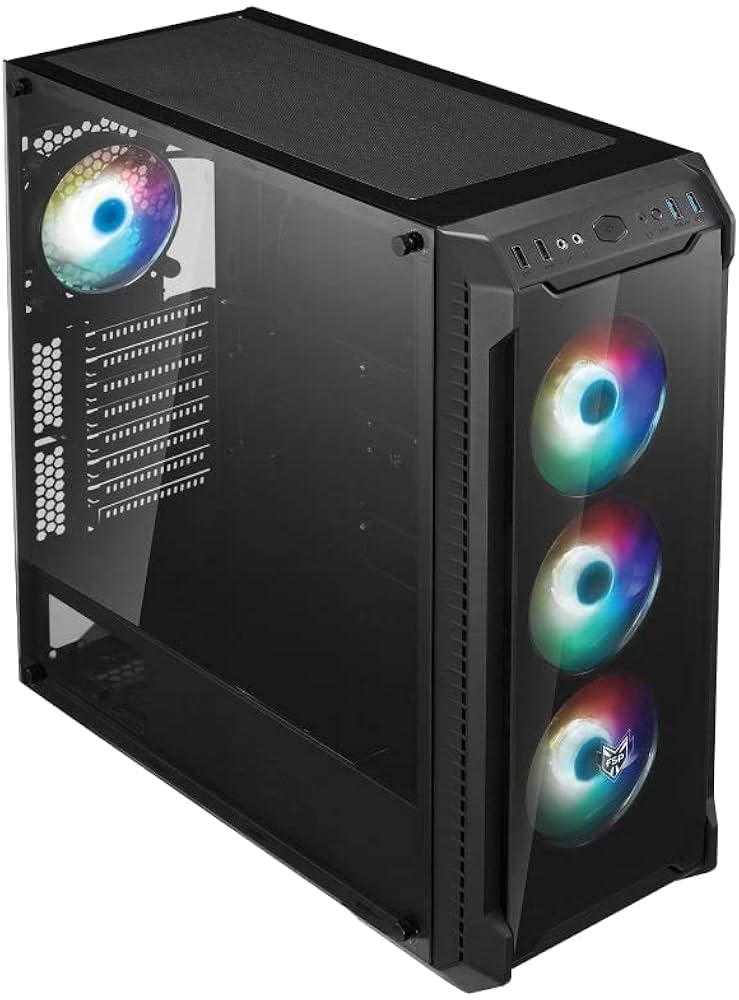
\includegraphics[width=3cm]{assets/img-desktop1.png} & AMD RYZEN 7 7800X CPU; RTX 5070 12G; 32 GB RAM DDR5 7200MHz; 1 TB NVMe SSD & Model training (AI Workload)\\
\hline
Workstation B (Desktop) & 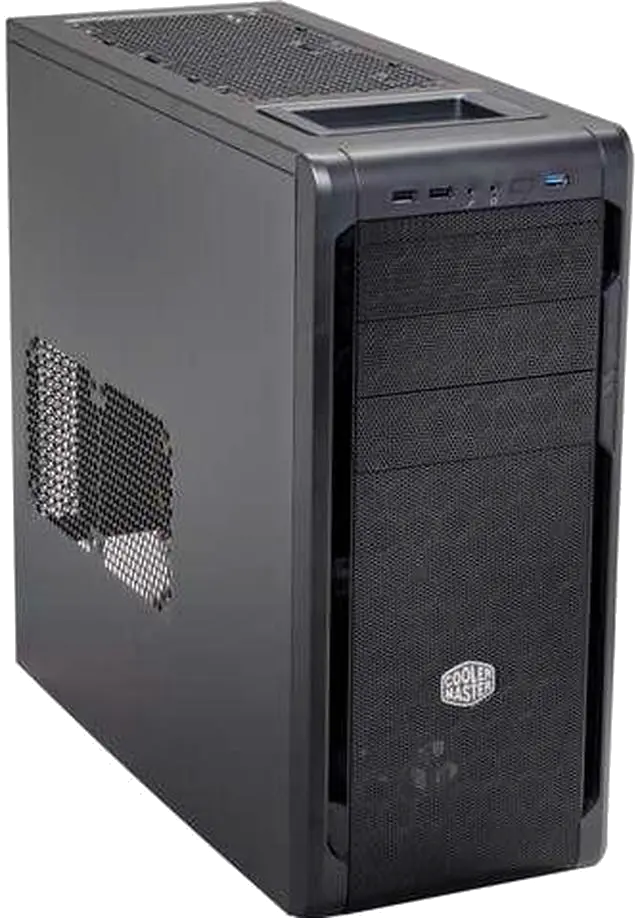
\includegraphics[width=3cm]{assets/img-desktop2.png} & Intel Core i7 6700K CPU; GTX 980 Ti; 16 GB RAM DDR4 3200MHz; 1 TB SATA SSD; 2 TB HDD & 3D Modeling, Video/Image Editing \\
\hline
ThinkPad T480 (Laptop) & 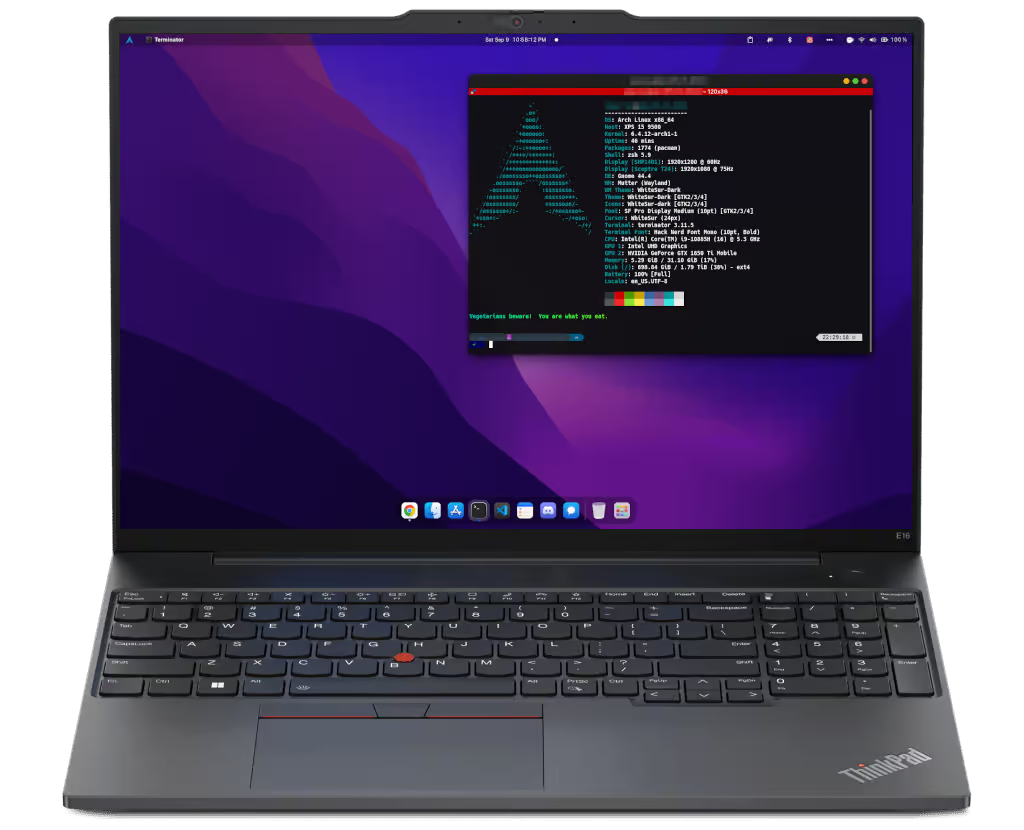
\includegraphics[width=3cm]{assets/img-laptop1.png} & Intel Core i5-8250U CPU; Integrated graphics; 8 GB RAM; 256GB NVMe SSD & Documentation \& Thesis Writing \\
\hline
ASUS Vivobook 17 (Laptop) & 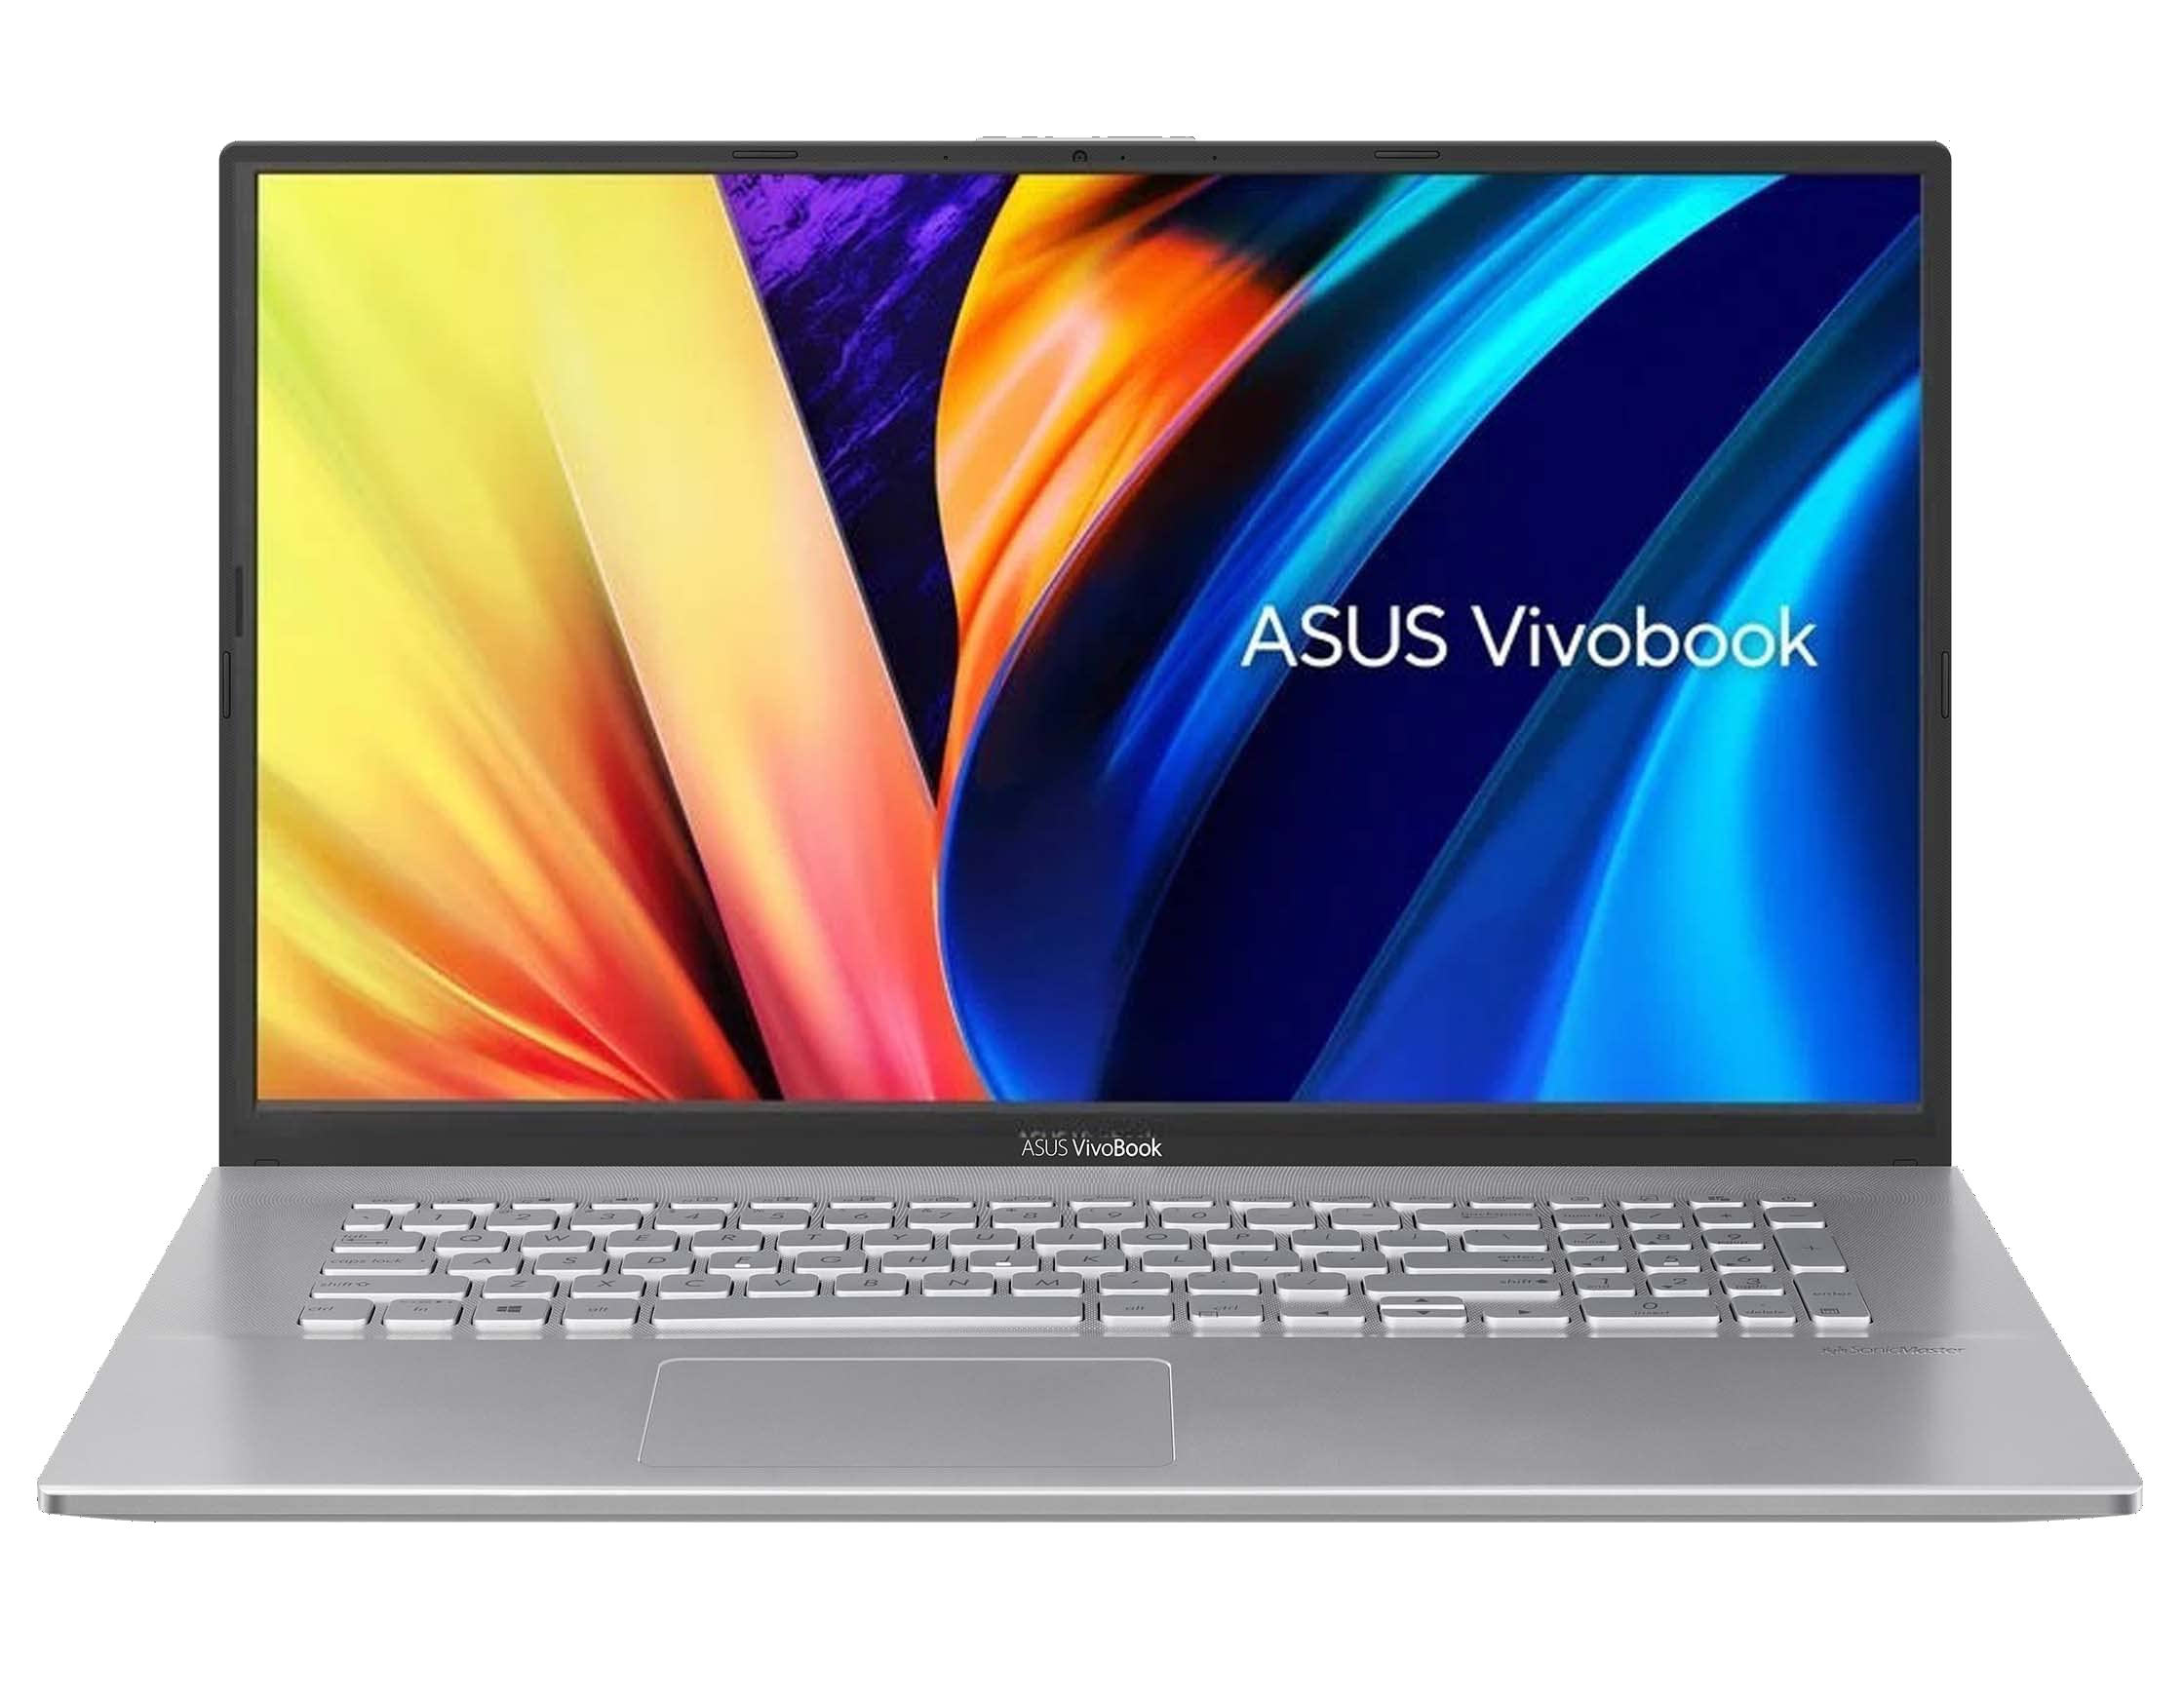
\includegraphics[width=3cm]{assets/img-laptop2.png} & Intel Core i7-8550U CPU; GTX 1050 4G; 16 GB DDR4 2400MHz; 256GB NVMe SSD; 1TB HDD & On-site demos and lightweight experiments \\
\hline
\end{tabular}
\end{table}
\indent Well, juggling four different workstations turns file syncing into a small saga: we relied on \textbf{GitHub} for versioned code, \textbf{LocalSend} and \textbf{Google Drive} for the large blobs, and the occasional \textbf{social-media DMs} (quick drag-and-drop) as a last-resort lifeline to keep things moving. The main training machine is an \textbf{AMD Ryzen 7 7800X} desktop with an \textbf{RTX 5070} GPU that chews through heavy Deep RL training workloads, while the other rigs handled \textbf{3D modeling}, \textbf{video/image editing}, and \textbf{writing}. To keep the chaos manageable we adopted lightweight \textbf{naming conventions} and frequent tiny \textbf{checkpoints}, which, together with a bit of coordination and luck, kept experiments reproducible and the team sane.
\clearpage
